\documentclass[12pt,a4paper]{article}
\usepackage{graphics}
\usepackage{amsmath}
\usepackage[english]{babel}
\usepackage{geometry}
\usepackage{hyperref}
\usepackage[utf8]{inputenc} 
\usepackage{listings}  
\usepackage{graphicx}
\usepackage{minted} 
\usepackage{hyperref} 
%\renewcommand{\thepart}{\roman{part}}
\usemintedstyle{default}
% Define a style for Python code
\lstset{
	language=Python,
	basicstyle=\ttfamily\small, % Font size and style
	keywordstyle=\color{blue}, % Keywords font color
	stringstyle=\color{orange}, % Strings font color
	commentstyle=\color{gray}, % Comments font color
	showstringspaces=false, % Don't show spaces in strings
	breaklines=true, % Wrap long lines
	numbers=left, % Show line numbers
	numberstyle=\tiny\color{gray}, % Line numbers font style
	frame=single, % Add a frame around the code
}

\title{\textbf{Building of spam detection's system based on SVM, LogisticRegession and Naive base, Machine learning algorithms}}
\author{Murhula Byabushi Christian}
\date{\today}


\begin{document}
	\maketitle  
	\newpage
	\listoffigures
	\tableofcontents
	\newpage
		
\part{Introduction}  
With the increasing of use of mobile devices and the rise of mobile communication, the number of text messages sent every day has grown exponentially. Along with this growth, there has been an increase in the number of spam messages being sent to users. Spams messages, also known as scams, are fraudulent messages that aim to deceive people into providing personal information, sending money, menacing to death or taking other actions that benefit the scammer.  \\

To address this problem, various techniques have been developed for detecting and filtering out spam messages on mobile devices. \\
One approach to spam detection on mobile devices is to use machine learning algorithms that analyze message content and metadata to determine wether a message is spam or not. In this article, we'll explore how machine learning can be used for spam detection, and show how to build a simple spam classifier using Python, we will use also a downloaded messages from \textit{Kaggle} environment, for reason of practices before investigating in a deep collection.\\ 

The first step in building a spam detector is to collect a dataset of emails that have been manually labeled as spam or not spam. The dataset should be split into training set and a test set, with the training set used to train the machine learning model and the test used to evaluate its performance.\\
Once the dataset is prepared, we can use machine learning algorithms to automatically classify emails as spam or not spam. Once common approach is to use a technique called text classification, where the content of the email is transformed into a numerical vector using a technique like the term frequency-inverse document frequency (TF-IDF) vectorizer. This vector is then used as input ot a machine learning algorithm, such as logistic regression, support vector machines (SVM), naive Bayes or neural networks. The algorithm learns from the training data to predict the correct class of new, unseen messages. 
\\

Any machine learning projects requires pursuing completely 5 steps as follows: Defining the object and specification, preparing and exploring the data, model building, implementation, testing, and deployment \cite{mlwithpython}. \\
\part{Methodology and practices}
\section{Defining the object and specification} 
This project consist of analyzing the dataset of mails present on Kaggle, that can be found inside of the at \url{https://www.kaggle.com/code/christianbyabushi/email-data-try/edit/run/122565281}, then building a system of predictions. 
For having an effective system of predictions and high accuracy, 3 models of machines are combined such as : Naive Bayes, Super Vector Machine and Logistic Regression. 
\\
In fact, combining multiple models and classification algorithms can boost the predictive
performance of an ML system even further \cite{raschka2017python}. different approaches are used, one of them is called : \textit{ensemble methods} . In the case of this work, we are going to use the \textit{VotingClassifier} method of sklearn python's package.
\section{Preparing and exploring the data}
Through this present step, an overview of dataset is given, all duplicates are removed, and inconsistent data are processed. In machine learning as much as the data is cleansed and abundant the as much as predictions are brights.\\
We have to install all dependencies beforehand and then import the data as follows:
\begin{minted}{python} 
#Install independencies
from sklearn.naive_bayes import MultinomialNB
from sklearn.svm import LinearSVC
from sklearn.linear_model import LogisticRegression
from sklearn.ensemble import VotingClassifier
from sklearn.feature_extraction.text import TfidfVectorizer
from sklearn.metrics import accuracy_score,
precision_score, recall_score, f1_score
from sklearn.model_selection import train_test_split
import numpy as np 
import pandas as pd

#The codes that serve to import now the data are follows:
data_email = pd.read_csv('mail_data.csv')  
#To get the simple overview of the dataset 
data_email.head() 
\end{minted} 
As Visualizing is considered as useful tool for data cleaning, exploring data structure, detecting outliers and unusual
groups, identifying trends and clusters, spotting local patterns, evaluating modeling output, and
presenting results \cite{unwin2020data}, let us deal with a set of codes for trend of the dataset at figure \ref{fig:imageOverviewDataset}.
\begin{minted}{python} 
# Counts the number of spams and hams
>> spam_output = data_email['Category'].to_numpy() 
numberOfham=0
numberOfSpam=0
for i in spam_output:
	if i=='ham':
		numberOfham+=1 
	else:
		numberOfSpam+=1 
counts = [numberOfham,numberOfSpam]
# create arrayofvalues
spam_output = data_email['Category'].to_numpy()

# create a bar chart
labels = ["Ham", "Spam"]
plt.bar(labels, counts)
plt.xlabel("Spam and Ham")
plt.ylabel("Number of message")
plt.title("Graphic of messages")
plt.show()
\end{minted}
\begin{figure}[htbp]
	\centering
	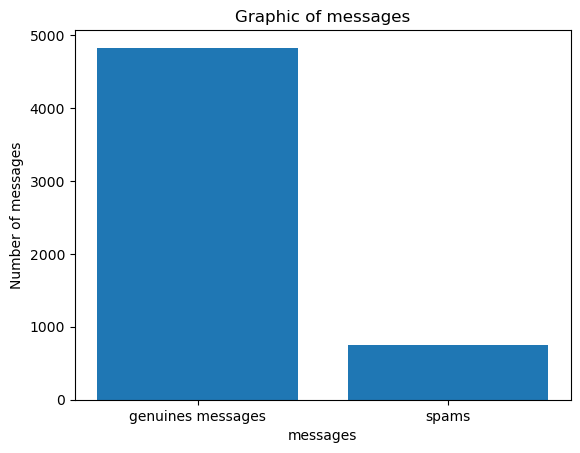
\includegraphics[width=0.8\textwidth]{../Spam/viewdataset}
	\caption{Overview of dataset}
	\label{fig:imageOverviewDataset}
\end{figure} 
classifying data in a proper format input prepare data for machine learning projects, in such way because labels are known, a supervised model can be used. On contrary, if the labels are unknown, the model to deal with must use clusters which can give a set of measurements, observations \cite{han2022data}.   
For the case of this work, the attributes or labels are available, thus we are going to use supervised models. Ultimately, let us classifying the dataset but spitting it in the clear format by defining the input and output labels the set of codes as follows:
\begin{minted}{python} 
#input
>> X = data_email['Message']
#output 
>> Y = data_email['Category']
\end{minted}
\section{Model building}
Model building refers to the process of creating a mathematical representation of a system or problem using data. The goal is to train the model on a set of input-output pairs, so that it can accurate predictions on new, unseen data \cite{introducgtionMlAlpay}. Therefore we are going to split in two separate ranges the (inputs and outputs), that we can store into the arrays by tuples. One part are labels for training models and others are for testing, as follows but the set of codes:
\begin{minted}{python}
>> x_train, x_test, y_train,y_test =
train_test_split(X,Y,test_size=0.2, random_state=3)
\end{minted}
It is considered that 80\% of data will serve for the training data and the rest for testing both for features and outputs. 
The random\_state parameter equalized to 3 as key, allows the algorithm to reproduce the same data as though the dataset is spitted more again.
\section{Feature Extraction }
Feature extraction is an important step in machine learning where relevant information is selected from raw data to be used in building a model \cite{fetAnjali2018}. For the case of this work, we use TfidfVectorizer, a common technique used in spam detection because it can convert textual data into numerical features that can be used in machine learning models based on natural language processing algorithms (NLPA). 
The term Tfdif inside stands for "Term Frequency-Inverse Document Frequency", which is a technique used to measure the importance of each word in a text corpus, an input for a NLPA.\\
How do we initialize a TFIDF in python ? 

\begin{minted}{python}
>> feature_extraction = TfidfVectorizer(min_df=1,
stop_words='english', lowercase =True)   
\end{minted}
- With the min\_df parameter, every word can be included inside of the object if it appears at least one time in the text;\\
- The stop\_words sets the word (commonly used in a language) that will be removed during the processing;\\
- The lowercase parameter sets all words in lowercase before the process.\\

The next process, is to define the feature space. What is it ?  
Before talking about the feature space, let us explain what is the feature vector.
A feature vector is a numerical vector that represents the features of an example in a dataset where each feature represents a specific piece of information about the example, which can be used to train a machine learning model. For example, in the case of the textual data, each feature may represent the number of occurrences of a specific word in the text, or TF-IDF score of that word \cite{introducgtionMlAlpay}.\\

Thus, the feature space is the set of all features vectors for all examples in a dataset. It is an abstract mathematical space that is defined by choice of features and the way they are transformed or normalized \cite{FeatuareSpaceSoltani}. In machine we usually train models on datasets that have been preprocessed into an appropriate feature space. This allows machine learning algorithms to process the data in a way that is more conducive to detecting relationships and patterns. \\
In addition, the data trained requires to be learned for detecting the vocabulary and the IDF (inverse document frequency) weights of the terms in the text corpus, by the object TfidfVectorizer, the set of codes as follows performs that task :
\begin{minted}{python}
>> x_train_features = feature_extraction.fit_transform(x_train) 
\end{minted}
Then, the same process is required for the test data, although this one will not be fitted, why ? because we want to the use the same feature space obtained when we fited the x\_train data. We must ensure that the test data is transformed into the same feature space as the training data, allowing for accurate comparison and evaluation of the model performance.
N.B: By using the new feature space obtained from x\_test, considered as our input can lead to potentially biased results, because we would be learning new vocabulary and IDF weights that were not present in the training data.

\section{Initializing Models for predictions}
In present work, three models are used for more accuracy, whereas they require the object that can combine all them. The below codes performs that tasks:
\begin{minted}{python}
#Naive Bayes
>>nb_model = MultinomialNB() 
#Suppor vector Machine
>>svm_model = LinearSVC()
#Logistic Regression
>>lr_model = LogisticRegression() 
	
#Model Whicn combines them
>>ensemble_model = VotingClassifier(estimators=[('nb',>>nb_model), 
('svm', svm_model), ('lr', lr_model)],>>voting='hard')
\end{minted}
Moreover, the dataset required to be fitted by the model. This process allows the it to learn the patterns and relationships between the input and the target variable, by creating a mathematical representation of the system. In python, with \textit{sklearn} package the fitting is performed as follows:
\begin{minted}{python}
>> ensemble_model.fit(x_train_features, y_train)
\end{minted}

\section{Evaluating the model}
Evaluating a model is an essential part of a machine learning project. The goal of model selection is to estimate how the model is expected to perform on new, previously unseen data.This is generally done by estimating its generalization error using the training set \cite{geron2022hands}. The library of sklearn that usually performs that tasks is metrics, initialized above.  
\begin{minted}{python}
#Evaluating models by predicting the test values and then compare to the y_test
# compute evaluation metrics 
>> predictions = ensemble_model.predict(x_test_features) 

>> acc_score = accuracy_score(y_test, predictions)
>> prec_score = precision_score(y_test, predictions, pos_label=0)
>> rec_score = recall_score(y_test, predictions, pos_label=0)
>> f1 = f1_score(y_test, predictions, pos_label=0) 
>> print("Accuracy score:", acc_score)
>> print("Precision score:", prec_score)
>> print("Recall score:", rec_score)
>> print("F1 score:", f1)
Accuracy score: 0.979372197309417
Precision score: 1.0
Recall score: 0.8516129032258064
F1 score: 0.9198606271777003
\end{minted} 
As a brief explanation of each functions used for evaluating the performance of a classification model: The first one, accuracy\_score: Computes the accuracy of a classification model by comparing the predicted labels to the true labels (\href{https://scikit-learn.org/stable/modules/generated/sklearn.metrics.accuracy_score.html}{link}).
\\The second, precision\_score: Computes the precision of a classification model by measuring the proportion of true positives (correctly predicted positive instances) among all instances that are predicted as positive (\href{https://scikit-learn.org/stable/modules/generated/sklearn.metrics.precision_score.html}{link}) . \\
The third, recall\_score: Computes the recall of a classification model by measuring the proportion of true positives among all actual positive instances (\href{https://scikit-learn.org/stable/modules/generated/sklearn.metrics.recall_score.html}{link}). and the last, f1\_score: Computes the F1 score of a classification model, which is the harmonic mean of precision and recall (\href{https://scikit-learn.org/stable/modules/generated/sklearn.metrics.f1_score.html}{link}). 

\section{Building a Predictive System}
By the below code, the system receives the input message and extract numerically for better processing and prediction by the ensembleModel object. The python are presented as follows : 
\begin{minted}{python}
>> input_text = input("Enter your mail here: ")
>> input_vector = feature_extraction.transform([input_text])
>> prediction = ensemble_model.predict(input_vector)[0]

>> if prediction == 0:
	print("This is a spam message")
>> else:
>>      print("This is not a spam message")
\end{minted}

\part{Conclusion}
In conclusion, we have built a spam detection system using three popular machine learning algorithms: SVM, Logistic Regression, and Naive Bayes. These algorithms were trained on a dataset of labeled spam and non-spam messages, and were evaluated using various metrics such as accuracy, precision, recall, and F1 score. The results showed that each algorithm had its strengths and weaknesses, and that combining the predictions of the three models led to a more accurate and robust spam detection system. Overall, this project demonstrates the power of machine learning in solving real-world problems and highlights the importance of careful evaluation and selection of algorithms in achieving optimal performance

\newpage
\bibliographystyle{plain}
\bibliography{bibfile.bib}

\end{document}
